\chapter{जीवित जगत का वर्गीकरण}\label{ch:b1:classifying-biodiversity}

लगभग \num{2} लाख हज़ार, यानी बीस लाख \omterm{def:b1:classifying-biodiversity:species}{जातियों} के नाम रखे जा चुके हैं, और
हर साल लगभग \num{18000} और जुड़ते हैं; जितनी हैं उनकी संख्या अकेले
\omterm{def:b1:cell-unit-of-life:prokeuk}{सुकेंद्रकियों} के लिए लगभग \num{9} लाख हज़ार आँकी जाती है, और बैक्टीरिया
कितने हैं यह किसी को पता नहीं। कोई नाम केवल शुरुआत है: कोई जीवविज्ञानी
जानना चाहता है कि कौन-सी \omterm{def:b1:classifying-biodiversity:species}{जाति} किसके सबसे पास है, और उत्तर एक वृक्ष है,
क्योंकि \omterm{def:b1:classifying-biodiversity:species}{जातियाँ} वंशक्रम से संबंधित हैं। यह अध्याय नामकरण के नियम देता है,
वे विधियाँ जिनसे लक्षणों से संबंध निकाले जाते हैं --- और वह कसौटी,
\omterm{def:b1:classifying-biodiversity:parsimony}{मितव्ययिता}, जिससे होड़ करते वृक्षों को परखा जाता है --- जीवन के वृक्ष का
वह आकार जैसा वह अब समझा जाता है, और जो कुछ जीता है उसकी सूची की हालत भी।

\section{जातियाँ और नाम}

\begin{definition}[जाति]\label{def:b1:classifying-biodiversity:species}
\index{जाति}\index{जैविक जाति संकल्पना}
\emph{जैविक जाति संकल्पना} के अंतर्गत कोई \emph{जाति} \omterm{def:b1:populations:population}{आबादियों} का ऐसा
समूह है जिसके सदस्य आपस में प्रजनन करके उपजाऊ संतति दे सकें और दूसरे ऐसे
समूहों से जननिक रूप से अलग हों। यह संकल्पना उन \omterm{def:b1:organism-environment:organism}{जीवों} पर लागू नहीं हो सकती
जो लैंगिक जनन नहीं करते (अधिकांश बैक्टीरिया, कई प्रोटिस्ट और कुछ पौधे तथा
जंतु), न जीवाश्मों पर, न ऐसी \omterm{def:b1:populations:population}{आबादियों} पर जो कभी मिलती ही नहीं; वहाँ कोई
जाति उसकी आकारिकी से (\emph{आकारिकीय} संकल्पना), किसी वृक्ष पर उसके
विशिष्ट वंशक्रम से (\emph{जातिवृत्तीय} संकल्पना), या जननिक विचलन की किसी
देहली से पहचानी जाती है। सारी संकल्पनाएँ एक ही चीज़ का नाम रखने की कोशिश
करती हैं: दूसरों से अलग होकर विकसित होता कोई वंशक्रम।
\end{definition}

\begin{definition}[नामपद्धति और कोटियाँ]\label{def:b1:classifying-biodiversity:nomenclature}
\index{द्विनाम नामपद्धति}\index{वर्गक}\index{वंश}\index{प्ररूप नमूना}
हर \omterm{def:b1:classifying-biodiversity:species}{जाति} का एक \emph{द्विनाम} होता है: उसके \emph{वंश} का नाम (बड़े अक्षर
से) और उसके बाद एक जातीय विशेषण, दोनों तिरछे अक्षरों में ---
\emph{Homo sapiens}, \emph{Quercus robur},
\emph{Escherichia coli} --- और अक्सर उसके बाद उसके वर्णन का लेखक तथा
वर्ष। यह पद्धति, जिसे लिनियस ने 1753 (पौधे) और 1758 (जंतु) में तय किया,
\omterm{def:b1:classifying-biodiversity:species}{जातियों} को \emph{कोटियों} के एक अनुक्रम में बसाती है: वंश, कुल, गण, वर्ग,
संघ (या प्रभाग), जगत, अधिजगत। किसी भी कोटि का समूह एक \emph{वर्गक} है। हर
नाम किसी \emph{प्ररूप नमूने} से बँधा होता है, जो किसी संग्रहालय या
हर्बेरियम में जमा रहता है और तय करता है कि वह नाम किसे इंगित करता है;
सबसे पुराने वैध नाम को वरीयता मिलती है; और नियम इस तरह संहिताबद्ध हैं कि
किसी एक \omterm{def:b1:organism-environment:organism}{जीव} का दुनिया भर में एक ही नाम हो। कोटियाँ रूढ़ियाँ हैं --- ऐसा
कोई गुण नहीं जो सारे कुल साझा करें और कोई वंश न करे; केवल \omterm{def:b1:classifying-biodiversity:species}{जाति} ही एक
प्राकृतिक इकाई है।
\end{definition}

\begin{omfigure}
\begin{tikzpicture}[font=\footnotesize, line cap=round]
  \draw[thick, omDef!60!black, fill=omDef!6, rounded corners=4pt] (0,0) rectangle (11.4,5.4); \node[anchor=north west, omDef!80!black] at (0.1,5.35) {अधिजगत यूकैरिया};
  \draw[thick, omDef!60!black, fill=omDef!10, rounded corners=4pt] (0.4,0.3) rectangle (11.0,4.75); \node[anchor=north west, omDef!80!black] at (0.5,4.7) {जगत ऐनिमेलिया};
  \draw[thick, omProp!70!black, fill=omProp!10, rounded corners=4pt] (0.8,0.6) rectangle (10.6,4.1); \node[anchor=north west, omProp!80!black] at (0.9,4.05) {संघ कॉर्डेटा};
  \draw[thick, omProp!70!black, fill=omProp!18, rounded corners=4pt] (1.2,0.9) rectangle (10.2,3.45); \node[anchor=north west, omProp!80!black] at (1.3,3.4) {वर्ग मैमेलिया};
  \draw[thick, omThm!70!black, fill=omThm!10, rounded corners=4pt] (1.6,1.2) rectangle (9.8,2.8); \node[anchor=north west, omThm!80!black] at (1.7,2.75) {गण कार्निवोरा};
  \draw[thick, omThm!70!black, fill=omThm!20, rounded corners=4pt] (2.0,1.4) rectangle (5.6,2.3); \node[anchor=north west, omThm!80!black] at (2.1,2.25) {कुल फ़ेलिडी};
  \node[anchor=west] at (2.1,1.65) {वंश \emph{Felis}: \emph{F.~catus}};
  \draw[thick, omThm!70!black, fill=omThm!20, rounded corners=4pt] (5.9,1.4) rectangle (9.5,2.3); \node[anchor=north west, omThm!80!black] at (6.0,2.25) {कुल कैनिडी};
  \node[anchor=west] at (6.0,1.65) {वंश \emph{Canis}: \emph{C.~lupus}};
\end{tikzpicture}

{\small बिल्ली और भेड़िए के लिए लिनियन अनुक्रम की बसी हुई कोटियाँ। हर
डिब्बा एक \omterm{def:b1:classifying-biodiversity:nomenclature}{वर्गक} है; द्विनाम \omterm{def:b1:classifying-biodiversity:nomenclature}{वंश} और \omterm{def:b1:classifying-biodiversity:species}{जाति} का नाम रखता है।}
\end{omfigure}

\begin{omfigure}
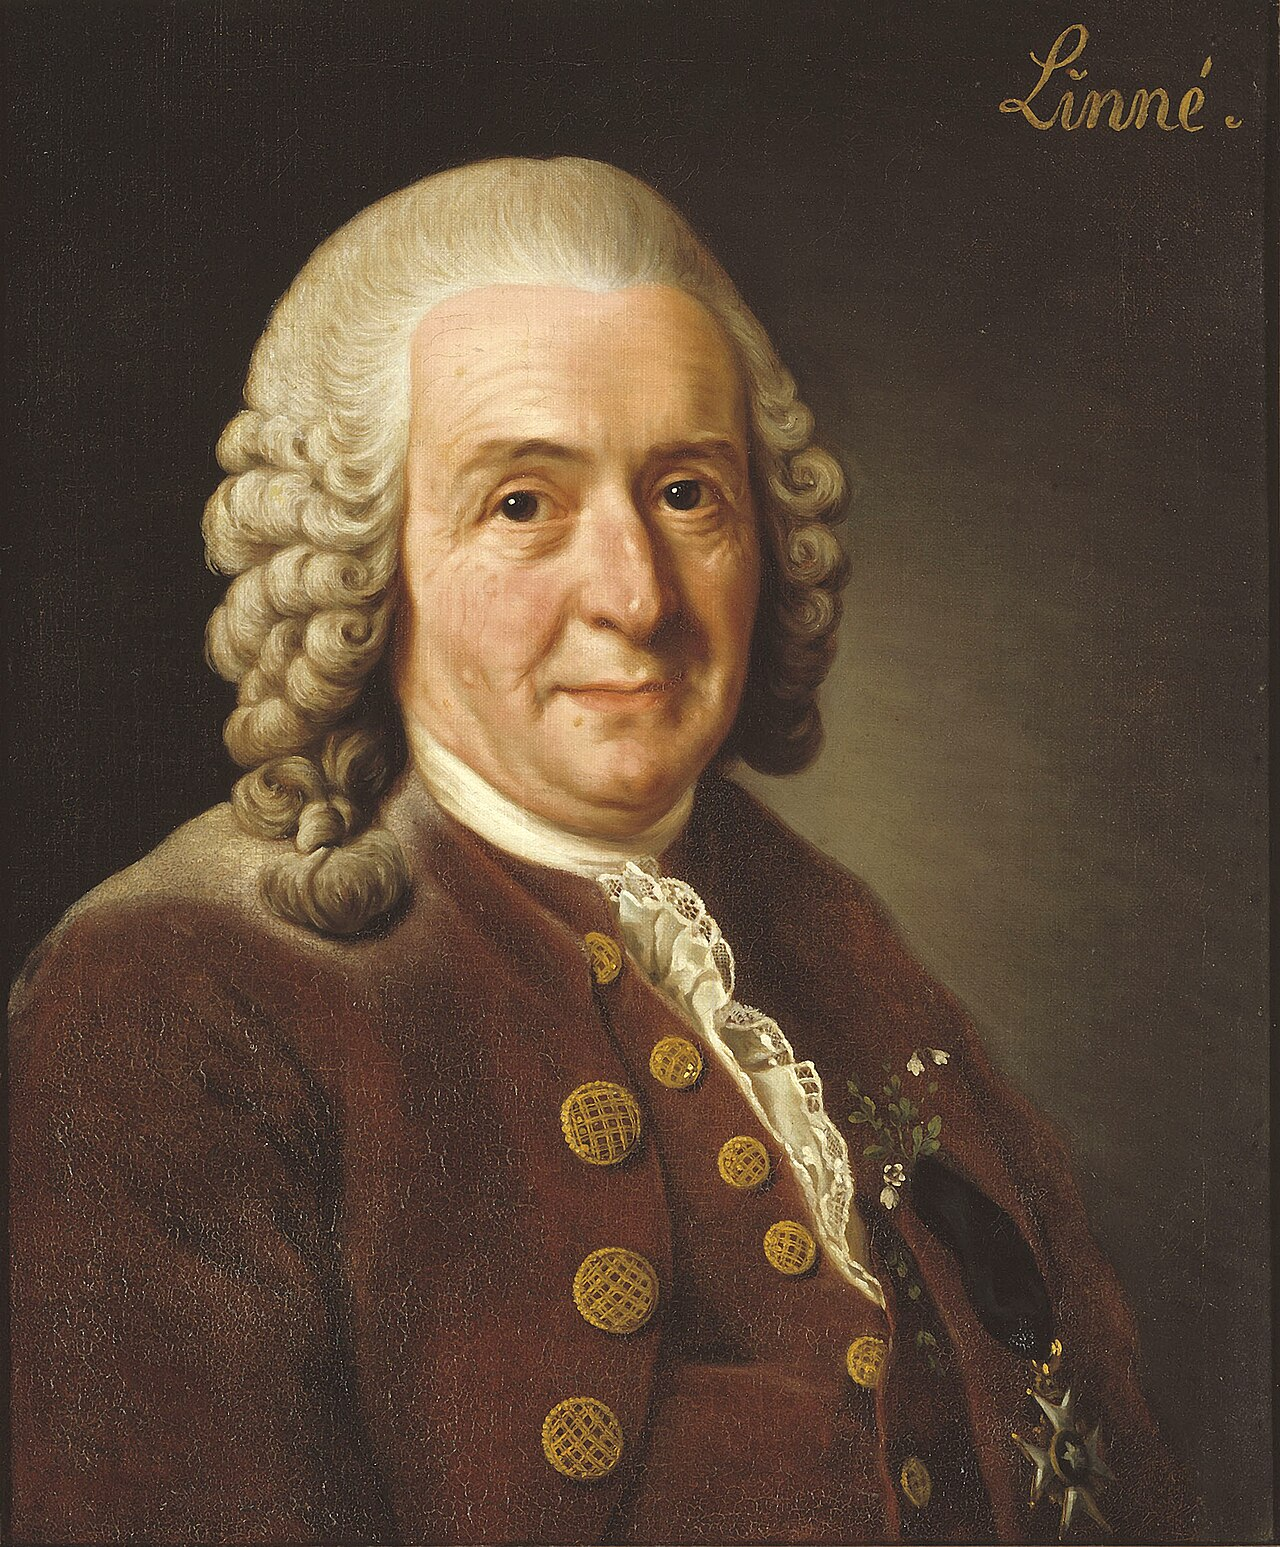
\includegraphics[width=0.36\linewidth]{images/book3/linnaeus.jpg}

{\small कार्ल लिनियस (1707--1778), जिनका 1753 का \emph{स्पीसीज़ प्लांटैरम}
और 1758 का \emph{सिस्टेमा नैचुरे} का दसवाँ संस्करण वानस्पतिक तथा
प्राणिशास्त्रीय नामपद्धति के आरंभ-बिंदु हैं। चित्र अलेक्ज़ांडर रोसलिन का,
1775।}
\end{omfigure}

\begin{omfigure}
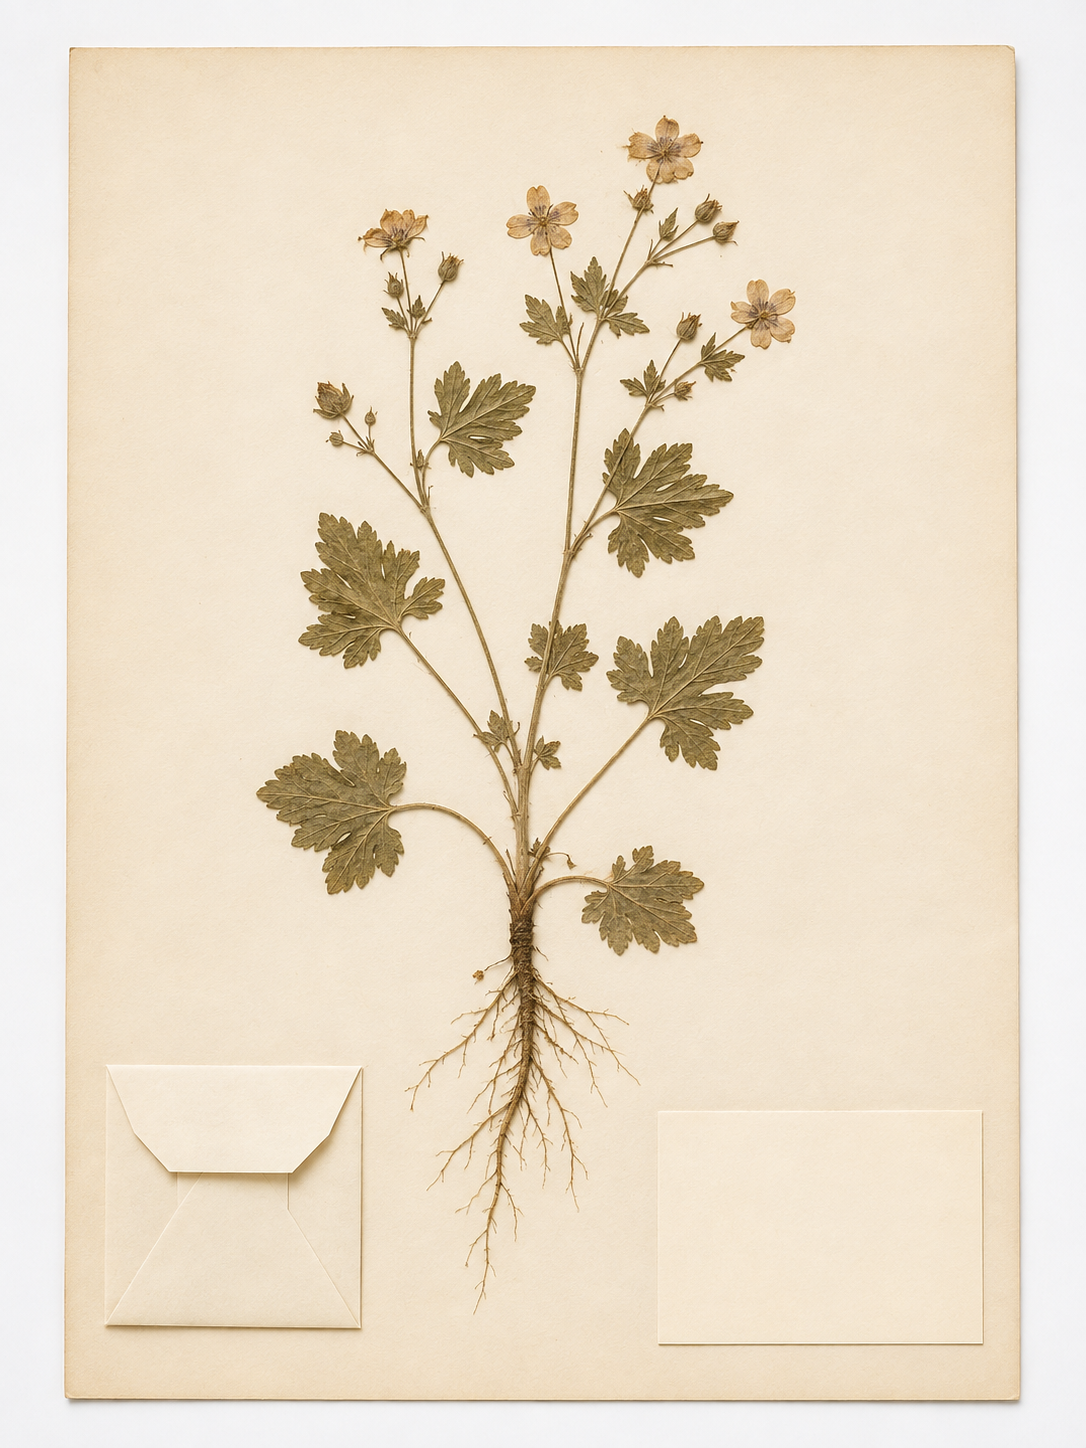
\includegraphics[width=0.5\linewidth]{images/book3/ai/b3-29-herbarium-sheet.png}

{\small एक हर्बेरियम पत्रक: दबाया हुआ, नामांकित नमूना, जैसा किसी पादप-नाम
के प्ररूप के रूप में और इस स्थायी साक्ष्य के रूप में काम आता है कि वह
\omterm{def:b1:classifying-biodiversity:species}{जाति} कहाँ और कब मिली थी।}
\end{omfigure}

\section{संबंधों का पुनर्निर्माण}

\begin{definition}[वर्गिकी, जातिवृत्त, क्लेडविज्ञान]\label{def:b1:classifying-biodiversity:systematics}
\index{वर्गिकी}\index{जातिवृत्त}\index{क्लेडविज्ञान}\index{क्लेड}
\emph{वर्गिकी} \omterm{def:b1:organism-environment:organism}{जीवों} की विविधता का और उनके आपसी संबंधों का अध्ययन है; कोई
\emph{जातिवृत्त} उन संबंधों का वृक्ष है, यानी इस बारे में एक परिकल्पना कि
वंशक्रम किस क्रम में बँटे। \emph{समलक्षणिकी} \omterm{def:b1:organism-environment:organism}{जीवों} को कुल मिलाकर समानता
से समूहबद्ध करती है और सारे लक्षण बराबर गिनती है; \emph{क्लेडविज्ञान}
उन्हें केवल साझे व्युत्पन्न लक्षणों से समूहबद्ध करता है, ताकि हर समूह एक
\emph{क्लेड} हो --- कोई पूर्वज और उसके सारे वंशज। आधुनिक वर्गीकरण का
लक्ष्य है कि हर नामित \omterm{def:b1:classifying-biodiversity:nomenclature}{वर्गक} एक क्लेड हो।
\end{definition}

\begin{definition}[लक्षण: समजातता, समवृत्तिता, ध्रुवता]\label{def:b1:classifying-biodiversity:characters}
\index{समजातता}\index{समवृत्तिता}\index{सहव्युत्पन्न लक्षण}\index{बाह्यसमूह}
कोई \emph{लक्षण} दो या अधिक \emph{अवस्थाओं} वाला कोई भी वंशागत गुण है
(अंग उपस्थित या अनुपस्थित; किसी \omterm{def:b1:genomes:gene}{जीन} में कोई दिया गया क्षारक A, C, G
या T)। दो \omterm{def:b1:organism-environment:organism}{जीवों} के लक्षण तब \emph{समजात} होते हैं जब वे किसी साझे पूर्वज
से वंशागत हों, और तब \emph{समवृत्त} जब वे अभिसरण या प्रत्यावर्तन से समान
हों (पक्षियों और चमगादड़ों के पंख; डॉलफ़िन और शार्क के धारारेखित शरीर)।
कोई लक्षण-अवस्था \emph{पैतृक} (पूर्वरूपी) है यदि वह समूह के पूर्वज में
मौजूद हो, और \emph{व्युत्पन्न} (उत्तररूपी) यदि वह समूह के भीतर उठी हो;
किसी \omterm{def:b1:classifying-biodiversity:systematics}{क्लेड} के साझे व्युत्पन्न लक्षण, यानी उसके \emph{सहव्युत्पन्न लक्षण},
ही उसके एकमात्र साक्ष्य हैं। ध्रुवता किसी \emph{बाह्यसमूह} से तुलना करके
तय होती है, यानी ऐसे \omterm{def:b1:classifying-biodiversity:nomenclature}{वर्गक} से जो निश्चित रूप से अध्ययन किए जा रहे समूह के
बाहर पड़ता है: वह जो अवस्था दिखाए उसे पैतृक माना जाता है।
\end{definition}

\begin{definition}[एकवंशजता, अपूर्णवंशजता, बहुवंशजता]\label{def:b1:classifying-biodiversity:monophyly}
\index{एकवंशजता}\index{अपूर्णवंशजता}\index{बहुवंशजता}
कोई समूह \emph{एकवंशज} (एक \omterm{def:b1:classifying-biodiversity:systematics}{क्लेड}) है यदि उसमें कोई पूर्वज और उसके सारे
वंशज हों; \emph{अपूर्णवंशज} यदि उसमें कोई पूर्वज और उसके केवल कुछ वंशज
हों (``सरीसृप'', जिनसे उन्हीं से उतरे पक्षी बाहर हैं; ``मछलियाँ'', जिनसे
चतुष्पाद बाहर हैं; ``अकशेरुकी''); और \emph{बहुवंशज} यदि वह किसी अभिसारी
लक्षण से अलग-अलग पूर्वजों के वंशजों को समूहबद्ध करे (``गरम-खून वाले
जंतु'', यानी पक्षी और स्तनधारी; ``शैवाल'')। अपूर्णवंशज समूह \omterm{def:b1:organism-environment:levels}{संगठन के
स्तरों} के उपयोगी वर्णन हैं पर \omterm{def:b1:classifying-biodiversity:systematics}{क्लेड} नहीं हैं और अब उन्हें औपचारिक नाम
नहीं दिए जाते।
\end{definition}

\begin{omfigure}
\begin{tikzpicture}[font=\footnotesize, line cap=round, >=Stealth]
  % tree: lamprey, shark, trout, lungfish, frog, lizard, bird, mammal
  \coordinate (r) at (6.5,-1.2);
  \draw[thick] (r) -- (6.5,-0.2);
  \draw[thick] (6.5,-0.2) -- (0.5,-0.2) -- (0.5,4.6); \node[anchor=south, rotate=60, anchor=west] at (0.5,4.6) {लैम्प्रे};
  \draw[thick] (6.5,-0.2) -- (6.5,0.6) -- (2.2,0.6) -- (2.2,4.6); \node[rotate=60, anchor=west] at (2.2,4.6) {शार्क};
  \draw[thick] (6.5,0.6) -- (6.5,1.3) -- (3.8,1.3) -- (3.8,4.6); \node[rotate=60, anchor=west] at (3.8,4.6) {ट्राउट};
  \draw[thick] (6.5,1.3) -- (6.5,2.0) -- (5.2,2.0) -- (5.2,4.6); \node[rotate=60, anchor=west] at (5.2,4.6) {फुफ्फुसमीन};
  \draw[thick] (6.5,2.0) -- (6.5,2.7) -- (6.6,2.7) -- (6.6,4.6); \node[rotate=60, anchor=west] at (6.6,4.6) {मेंढक};
  \draw[thick] (6.5,2.7) -- (8.7,2.7) -- (8.7,3.3);
  \draw[thick] (8.7,3.3) -- (8.0,3.3) -- (8.0,4.6); \node[rotate=60, anchor=west] at (8.0,4.6) {स्तनधारी};
  \draw[thick] (8.7,3.3) -- (9.7,3.3) -- (9.7,3.9);
  \draw[thick] (9.7,3.9) -- (9.3,3.9) -- (9.3,4.6); \node[rotate=60, anchor=west] at (9.3,4.6) {छिपकली};
  \draw[thick] (9.7,3.9) -- (10.6,3.9) -- (10.6,4.6); \node[rotate=60, anchor=west] at (10.6,4.6) {पक्षी};
  % groupings
  \draw[very thick, omDef, rounded corners=6pt] (7.6,3.05) rectangle (11.0,5.9); \node[omDef!80!black, anchor=south west] at (7.65,5.9) {उल्बधारी: एकवंशज};
  \draw[very thick, omThm, dashed, rounded corners=6pt] (9.0,3.6) -- (9.0,5.8) -- (10.15,5.8) -- (10.15,3.6) -- cycle; \node[omThm!80!black, anchor=west, align=left] at (11.1,4.8) {पक्षियों के बिना\\ ``सरीसृप'':\\ अपूर्णवंशज};
  \draw[very thick, omProp!80!black, dotted, rounded corners=6pt] (7.7,6.35) -- (7.7,6.8) -- (11.0,6.8) -- (11.0,6.35); \node[omProp!80!black, anchor=south] at (9.35,6.85) {``गरम-खून वाले'' (स्तनधारी $+$ पक्षी): बहुवंशज};
  \draw[very thick, gray, dashed, rounded corners=6pt] (1.8,4.3) -- (1.8,5.75) -- (5.7,5.75) -- (5.7,4.3); \node[gray, anchor=south] at (3.75,5.9) {चतुष्पादों के बिना ``मछलियाँ'': अपूर्णवंशज};
  % synapomorphies
  \node[font=\scriptsize, anchor=east] at (6.4,0.2) {जबड़े}; \draw[thick] (6.35,0.2) -- (6.65,0.2);
  \node[font=\scriptsize, anchor=east] at (6.4,0.95) {अस्थिल कंकाल}; \draw[thick] (6.35,0.95) -- (6.65,0.95);
  \node[font=\scriptsize, anchor=east] at (6.4,1.65) {फेफड़े}; \draw[thick] (6.35,1.65) -- (6.65,1.65);
  \node[font=\scriptsize, anchor=east] at (6.4,2.35) {चार अंग}; \draw[thick] (6.35,2.35) -- (6.65,2.35);
  \node[font=\scriptsize, anchor=west] at (8.8,2.82) {उल्ब अंडा}; \draw[thick] (8.55,2.82) -- (8.85,2.82);
\end{tikzpicture}

{\small आठ कशेरुकियों का एक क्लेडोग्राम, जिसकी शाखाओं पर \omterm{def:b1:classifying-biodiversity:characters}{सहव्युत्पन्न
लक्षण} अंकित हैं। \omterm{def:b1:classifying-biodiversity:systematics}{क्लेड} एकवंशज होते हैं; ``मछलियाँ'' और ``सरीसृप''
अपूर्णवंशज स्तर हैं; ``गरम-खून वाले जंतु'' किसी अभिसारी लक्षण से बना एक
बहुवंशज समूहन है।}
\end{omfigure}

\begin{definition}[मितव्ययिता]\label{def:b1:classifying-biodiversity:parsimony}
\index{मितव्ययिता}\index{वृक्ष-लंबाई}
\omterm{def:b1:classifying-biodiversity:nomenclature}{वर्गकों} के किसी समुच्चय को जोड़ सकने वाले सारे वृक्षों में
\emph{सबसे मितव्ययी} वह है जो लक्षण-अवस्था के सबसे कम विकासीय बदलाव
माँगता है --- यानी सबसे छोटी \emph{वृक्ष-लंबाई}, जो उस वृक्ष पर हर लक्षण
को चाहिए न्यूनतम बदलावों का लक्षणों भर योग है। जो लक्षण वृक्ष में एक ही
बदलाव से बैठ जाए वह उससे संगत है; जिसे दो या अधिक चाहिए वह उस वृक्ष पर एक
\omterm{def:b1:classifying-biodiversity:characters}{समवृत्तिता} है। मितव्ययिता यह दावा नहीं है कि विकास मितव्ययी है; वह यह
नियम है कि किसी परिकल्पना को अभिसरणों की संख्या आँकड़ों की मजबूरी से आगे
नहीं बढ़ानी चाहिए।
\end{definition}

\begin{method}[किसी लक्षण-आव्यूह से कोई क्लेडोग्राम बनाना]\label{met:b1:classifying-biodiversity:cladogram}
\begin{enumerate}
  \item \omterm{def:b1:classifying-biodiversity:nomenclature}{वर्गक} और एक \omterm{def:b1:classifying-biodiversity:characters}{बाह्यसमूह} चुनिए; लक्षणों को उनकी अवस्थाओं के साथ
        सूचीबद्ध कीजिए, \omterm{def:b1:classifying-biodiversity:characters}{बाह्यसमूह} की अवस्था को 0 (पैतृक) और व्युत्पन्न
        अवस्था को 1 कूटबद्ध करते हुए।
  \item \omterm{def:b1:classifying-biodiversity:nomenclature}{वर्गकों} को साझी व्युत्पन्न अवस्थाओं से समूहबद्ध कीजिए, उस लक्षण
        से शुरू करके जिसे सबसे अधिक \omterm{def:b1:classifying-biodiversity:nomenclature}{वर्गक} साझा करते हैं (सबसे गहरा
        \omterm{def:b1:classifying-biodiversity:systematics}{क्लेड}) और भीतर की ओर बसाते हुए; \omterm{def:b1:classifying-biodiversity:nomenclature}{वर्गकों} के किसी समुच्चय द्वारा
        साझा हर 1 उस समुच्चय के लिए एक संभावित \omterm{def:b1:classifying-biodiversity:characters}{सहव्युत्पन्न लक्षण} है।
  \item जहाँ लक्षण टकराएँ (दो समूहन दोनों \omterm{def:b1:classifying-biodiversity:systematics}{क्लेड} नहीं हो सकते), वहाँ हर
        विकल्प-वृक्ष खींचिए और उसकी लंबाई गिनिए: हर लक्षण के लिए वे कम
        से कम बदलाव जो उसकी अवस्थाएँ वृक्ष पर रख दें।
  \item सबसे छोटा वृक्ष रखिए; उस पर जिन लक्षणों को अतिरिक्त बदलाव चाहिए
        थे वही समवृत्तिताएँ हैं। यदि दो वृक्ष बराबर हों, तो आँकड़े तय
        नहीं करते और और लक्षण चाहिए।
  \item वृक्ष पढ़िए: क्लेडों के नाम रखिए, ध्यान दीजिए कि कौन-से पारंपरिक
        समूह अपूर्णवंशज हैं, और जाँचिए कि वह स्वतंत्र आँकड़ों (आणविक
        अनुक्रम, जीवाश्म) से मेल खाता है।
\end{enumerate}
\end{method}

\begin{example}[दो वृक्ष, गिने हुए]\label{ex:b1:classifying-biodiversity:count}
चार \omterm{def:b1:classifying-biodiversity:nomenclature}{वर्गक}: छिपकली, पक्षी, स्तनधारी, मेंढक (\omterm{def:b1:classifying-biodiversity:characters}{बाह्यसमूह})। लक्षण: उल्ब अंडा
(छिपकली, पक्षी, स्तनधारी: 1), द्विगर्ती खोपड़ी (छिपकली,
पक्षी), ऊष्मारक्तता (पक्षी, स्तनधारी)। वृक्ष A, (छिपकली, पक्षी) फिर स्तनधारी:
अंडा 1 बदलाव, खोपड़ी 1, ऊष्मारक्तता 2 (दो बार उठती) --- लंबाई 4।
वृक्ष B, (पक्षी, स्तनधारी) फिर छिपकली: अंडा 1, ऊष्मारक्तता 1, खोपड़ी 2 ---
लंबाई 4। बराबरी; टाँगों के शल्कों पर पंख और अधिचर्मी
शल्क (छिपकली, पक्षी) जोड़िए: वृक्ष A की लंबाई 5, वृक्ष B की 6। वृक्ष A
वरीय है, और ऊष्मारक्तता एक \omterm{def:b1:classifying-biodiversity:characters}{समवृत्तिता} है: वह दो बार विकसित हुई।
\end{example}

\begin{omfigure}
\begin{tikzpicture}[font=\footnotesize, line cap=round]
  \begin{scope}
    \draw[thick] (2.0,0) -- (2.0,0.8);
    \draw[thick] (2.0,0.8) -- (0,0.8) -- (0,3.0); \node[anchor=south] at (0,3.0) {मेंढक};
    \draw[thick] (2.0,0.8) -- (2.0,1.6) -- (1.2,1.6) -- (1.2,3.0); \node[anchor=south] at (1.2,3.0) {स्तनधारी};
    \draw[thick] (2.0,1.6) -- (3.0,1.6) -- (3.0,2.3);
    \draw[thick] (3.0,2.3) -- (2.4,2.3) -- (2.4,3.0); \node[anchor=south] at (2.4,3.0) {छिपकली};
    \draw[thick] (3.0,2.3) -- (3.6,2.3) -- (3.6,3.0); \node[anchor=south] at (3.6,3.0) {पक्षी};
    \draw[very thick, omDef] (1.85,1.2) -- (2.15,1.2); \node[anchor=east, font=\scriptsize, omDef!80!black] at (1.8,1.2) {अंडा};
    \draw[very thick, omDef] (2.85,1.95) -- (3.15,1.95); \node[anchor=west, font=\scriptsize, omDef!80!black] at (3.2,1.95) {खोपड़ी, शल्क};
    \draw[very thick, omThm] (1.05,2.5) -- (1.35,2.5); \node[anchor=east, font=\scriptsize, omThm] at (1.0,2.5) {ऊष्मारक्त};
    \draw[very thick, omThm] (3.45,2.65) -- (3.75,2.65); \node[anchor=west, font=\scriptsize, omThm] at (3.8,2.65) {ऊष्मारक्त};
    \node[anchor=north, align=center] at (1.9,-0.2) {वृक्ष A: लंबाई 5\\ (ऊष्मारक्तता दो बार)};
  \end{scope}
  \begin{scope}[xshift=7.4cm]
    \draw[thick] (2.0,0) -- (2.0,0.8);
    \draw[thick] (2.0,0.8) -- (0,0.8) -- (0,3.0); \node[anchor=south] at (0,3.0) {मेंढक};
    \draw[thick] (2.0,0.8) -- (2.0,1.6) -- (1.2,1.6) -- (1.2,3.0); \node[anchor=south] at (1.2,3.0) {छिपकली};
    \draw[thick] (2.0,1.6) -- (3.0,1.6) -- (3.0,2.3);
    \draw[thick] (3.0,2.3) -- (2.4,2.3) -- (2.4,3.0); \node[anchor=south] at (2.4,3.0) {स्तनधारी};
    \draw[thick] (3.0,2.3) -- (3.6,2.3) -- (3.6,3.0); \node[anchor=south] at (3.6,3.0) {पक्षी};
    \draw[very thick, omDef] (1.85,1.2) -- (2.15,1.2); \node[anchor=east, font=\scriptsize, omDef!80!black] at (1.8,1.2) {अंडा};
    \draw[very thick, omDef] (2.85,1.95) -- (3.15,1.95); \node[anchor=west, font=\scriptsize, omDef!80!black] at (3.2,1.95) {ऊष्मारक्त};
    \draw[very thick, omThm] (1.05,2.5) -- (1.35,2.5); \node[anchor=east, font=\scriptsize, omThm, align=right] at (1.0,2.5) {खोपड़ी,\\ शल्क};
    \draw[very thick, omThm] (3.45,2.65) -- (3.75,2.65); \node[anchor=west, font=\scriptsize, omThm, align=left] at (3.8,2.65) {खोपड़ी,\\ शल्क};
    \node[anchor=north, align=center] at (1.9,-0.2) {वृक्ष B: लंबाई 6\\ (खोपड़ी और शल्क दो बार)};
  \end{scope}
\end{tikzpicture}

{\small \omterm{def:b1:classifying-biodiversity:parsimony}{मितव्ययिता} दो वृक्षों के बीच यह गिनकर तय करती है कि हर एक कितने
बदलाव माँगता है। वृक्ष A को एक \omterm{def:b1:classifying-biodiversity:characters}{समवृत्तिता} चाहिए (ऊष्मारक्तता दो बार
उठती); वृक्ष B को दो; वृक्ष A रखा जाता है।}
\end{omfigure}

\begin{remark}[आणविक लक्षण]\label{rem:b1:classifying-biodiversity:molecular}
कोई जीन-अनुक्रम एक साथ सैकड़ों लक्षण देता है, हर स्थल चार अवस्थाओं वाला
एक लक्षण, जो ऐसे \omterm{def:b1:organism-environment:organism}{जीवों} के बीच भी तुलनीय है जो कोई दृश्य गुण साझा नहीं
करते --- कोई बैक्टीरियम और कोई बलूत। अनुक्रम पंक्तिबद्ध किए जाते हैं,
समजात स्थलों की तुलना की जाती है, और वृक्ष \omterm{def:b1:classifying-biodiversity:parsimony}{मितव्ययिता} से या ऐसी
सांख्यिकीय विधियों से बनाए जाते हैं जो प्रतिस्थापन की दर का प्रतिरूपण
करती हैं; आणविक घड़ी, यानी वह दर जिससे उदासीन अंतर जमा होते हैं, विभाजनों
की तिथि देती है। ये विधियाँ, और लंबी शाखाओं तथा असमान दरों के खतरे,
वर्ष 2 के खंड में लिए जाते हैं।
\end{remark}

\section{जीवन का वृक्ष}

\begin{proposition}[तीन अधिजगत]\label{prop:b1:classifying-biodiversity:domains}
\index{अधिजगत}\index{आर्किया}\index{बैक्टीरिया}\index{यूकैरिया}
जीवन तीन अधिजगतों में बँटता है: \emph{बैक्टीरिया}, \emph{आर्किया} और
\emph{यूकैरिया}। बैक्टीरिया और आर्किया दोनों कोशिका-संगठन में
\omterm{def:b1:cell-unit-of-life:prokeuk}{प्राक्केंद्रकी} हैं (\cref{ch:b1:cell-unit-of-life}) पर अपनी
झिल्ली-वसाओं, कोशिका-भित्तियों, \omterm{def:b1:nucleic-acids:chain}{RNA} पॉलिमरेज़ों और \omterm{def:b1:gene-expression:ribosome}{राइबोसोमों} में भिन्न
हैं; आर्किया के अनुलेखन तथा अनुवाद का तंत्र बैक्टीरिया के तंत्र की
तुलना में \omterm{def:b1:cell-unit-of-life:prokeuk}{सुकेंद्रकियों} के तंत्र के अधिक पास है, और \omterm{def:b1:cell-unit-of-life:prokeuk}{सुकेंद्रकी कोशिका}
किसी ऐसे आर्कियल वंशक्रम से उठी जिसने किसी बैक्टीरियम को अपना
\omterm{def:b1:eukaryotic-cell:mitochondrion}{सूत्रकणिका} बना लिया (\cref{ch:b1:eukaryotic-cell})। यूकैरिया के भीतर
पुराने जगत --- जंतु, पौधे, कवक और एक ``प्रोटिस्ट'' अवशेष ---
कुछ ही बड़े वंशक्रमों से बदल दिए जाते हैं, जिनमें जंतु, कवक और थलीय पौधे
तीन छोटी टहनियाँ हैं, और ``प्रोटिस्ट'' बाकी सब का एक अपूर्णवंशज जमावड़ा।
\end{proposition}
\begin{proof}[साक्ष्य]
वोइस और फ़ॉक्स (1977) ने लघु-उपइकाई \omterm{def:b1:nucleic-acids:rnas}{राइबोसोमी RNA} --- ऐसा अणु जो हर
\omterm{def:b1:cell-unit-of-life:cell}{कोशिका} में है, एक ही कार्य का और सारे जीवन भर पंक्तिबद्ध किया जा सकने
वाला --- का अनुक्रम बैक्टीरिया, मेथैनोजनों और \omterm{def:b1:cell-unit-of-life:prokeuk}{सुकेंद्रकियों} के बीच
मिलाया, और पाया कि मेथैनोजन बाकी बैक्टीरिया से उतने ही भिन्न थे जितना
इनमें से कोई \omterm{def:b1:cell-unit-of-life:prokeuk}{सुकेंद्रकियों} से। \omterm{def:b1:cell-unit-of-life:prokeuk}{प्राक्केंद्रकी} दो समूह थे, एक नहीं; और इस
एक \omterm{def:b1:genomes:gene}{जीन} से खींचा गया वृक्ष समूचे \omterm{def:b1:genomes:genome}{जीनोमों} से तथा आर्किया की विशिष्ट
जैवरसायनिकी (ईथर-बद्ध \omterm{def:b1:lipids:fattyacid}{लिपिड}, कोई पेप्टिडोग्लाइकन नहीं) से पुष्ट हो चुका
है।
\end{proof}

\begin{omfigure}
\begin{tikzpicture}[font=\footnotesize, line cap=round]
  \coordinate (root) at (5.0,0);
  \draw[very thick] (root) -- (5.0,1.0);
  \draw[very thick, omExo!80!black] (5.0,1.0) -- (1.6,1.0) -- (1.6,2.4);
  \draw[very thick, omExo!80!black] (1.6,2.4) -- (0.4,2.4) -- (0.4,3.6); \draw[very thick, omExo!80!black] (1.6,2.4) -- (1.6,3.6); \draw[very thick, omExo!80!black] (1.6,2.4) -- (2.8,2.4) -- (2.8,3.6);
  \node[anchor=south, rotate=60, anchor=west] at (0.4,3.6) {प्रोटियोबैक्टीरिया}; \node[rotate=60, anchor=west] at (1.6,3.6) {सायनोबैक्टीरिया}; \node[rotate=60, anchor=west] at (2.8,3.6) {ग्राम-धनी};
  \node[omExo!80!black, font=\small, anchor=north] at (1.6,0.9) {बैक्टीरिया};
  \draw[very thick] (5.0,1.0) -- (7.6,1.0) -- (7.6,1.7);
  \draw[very thick, omProp!80!black] (7.6,1.7) -- (5.8,1.7) -- (5.8,2.4);
  \draw[very thick, omProp!80!black] (5.8,2.4) -- (5.0,2.4) -- (5.0,3.6); \draw[very thick, omProp!80!black] (5.8,2.4) -- (6.6,2.4) -- (6.6,3.6);
  \node[rotate=60, anchor=west] at (5.0,3.6) {मेथैनोजन}; \node[rotate=60, anchor=west] at (6.6,3.6) {लवणरागी};
  \node[omProp!80!black, font=\small, anchor=north] at (5.8,1.6) {आर्किया};
  \draw[very thick, omDef] (7.6,1.7) -- (9.6,1.7) -- (9.6,2.4);
  \draw[very thick, omDef] (9.6,2.4) -- (8.0,2.4) -- (8.0,3.6); \draw[very thick, omDef] (9.6,2.4) -- (9.0,2.4) -- (9.0,3.6); \draw[very thick, omDef] (9.6,2.4) -- (10.0,2.4) -- (10.0,3.6); \draw[very thick, omDef] (9.6,2.4) -- (11.0,2.4) -- (11.0,3.6);
  \node[rotate=60, anchor=west] at (8.0,3.6) {थलीय पौधे, शैवाल}; \node[rotate=60, anchor=west] at (9.0,3.6) {कवक}; \node[rotate=60, anchor=west] at (10.0,3.6) {जंतु}; \node[rotate=60, anchor=west] at (11.0,3.6) {कई प्रोटिस्ट वंशक्रम};
  \node[omDef!80!black, font=\small, anchor=north] at (9.6,1.6) {यूकैरिया};
  \draw[->, thick, gray, dashed] (1.6,2.0) to[out=0, in=180] (9.6,2.1); \node[gray, font=\scriptsize, anchor=west] at (5.2,0.5) {कोई बैक्टीरियम सूत्रकणिका बन गया};
  \node[anchor=north] at (5.0,-0.1) {अंतिम सार्वत्रिक साझा पूर्वज};
\end{tikzpicture}

{\small \omterm{def:b1:nucleic-acids:rnas}{राइबोसोमी RNA} से निकले तीन अधिजगत। आर्किया \omterm{def:b1:cell-unit-of-life:prokeuk}{सुकेंद्रकियों} के
अधिक निकट संबंधी हैं, और \omterm{def:b1:cell-unit-of-life:prokeuk}{सुकेंद्रकी कोशिका} एक संगलन है: बैक्टीरियल
\omterm{def:b1:eukaryotic-cell:mitochondrion}{सूत्रकणिका} वाला कोई आर्कियल पोषी (और पौधों तथा शैवाल में एक दूसरा
बैक्टीरियल साझेदार, \omterm{def:b1:eukaryotic-cell:plastid}{हरितलवक})।}
\end{omfigure}

\begin{omfigure}
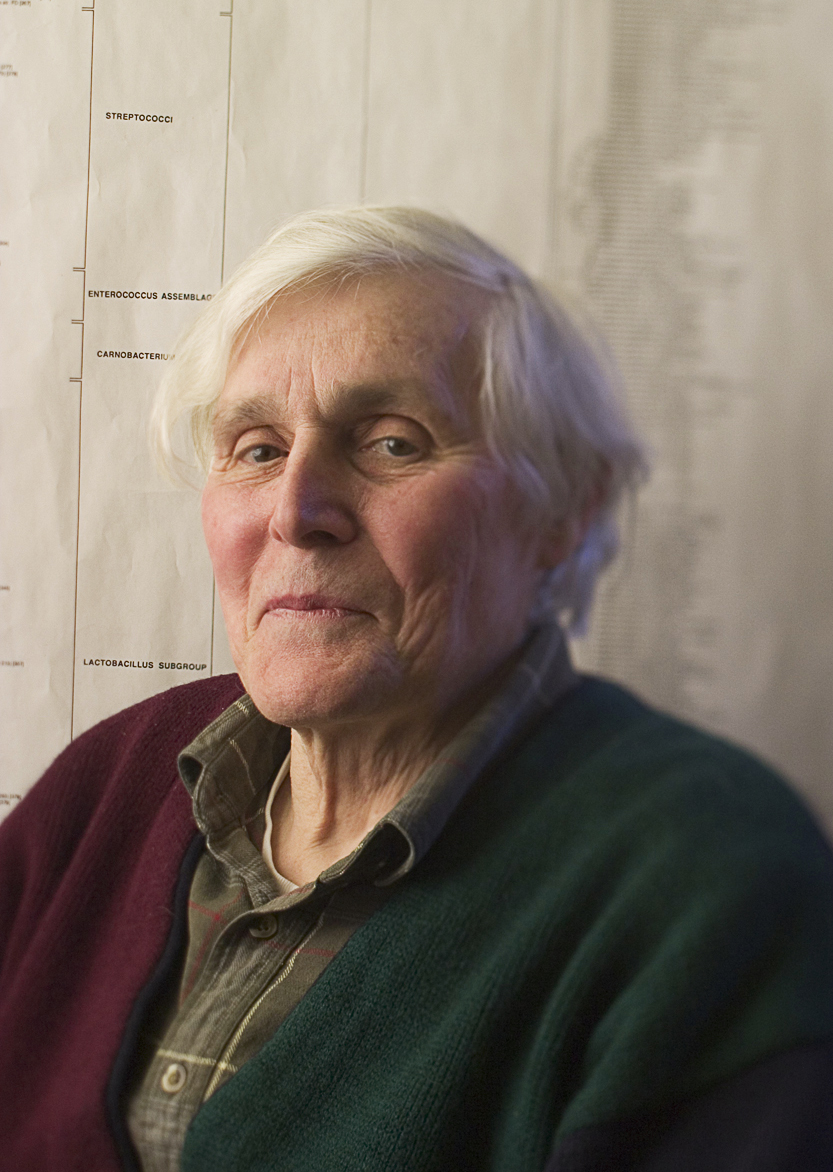
\includegraphics[width=0.34\linewidth]{images/book3/woese.jpg}

{\small कार्ल वोइस (1928--2012), बैक्टीरिया के किसी राइबोसोमी-RNA वृक्ष
के सामने। सारे जीवन भर इस एक ही अणु की उनकी तुलना ने आर्किया उजागर किए
और जीवन के वृक्ष को उसके तीन अधिजगत दिए।}
\end{omfigure}

\begin{proposition}[सुकेंद्रकियों के मुख्य वंशक्रम]\label{prop:b1:classifying-biodiversity:eukaryotes}
\omterm{def:b1:cell-unit-of-life:prokeuk}{सुकेंद्रकी} कुछ ही बड़े समूहों में आते हैं: \emph{ऑपिस्थोकॉन्ट}
(जंतु, कवक और उनके एककोशिकीय संबंधी, जिनकी \omterm{def:b1:cell-unit-of-life:cell}{कोशिकाएँ} एक ही पिछले कशाभ से
तैरती हैं); \emph{आर्किप्लास्टिडा} (थलीय पौधे,
हरे और लाल शैवाल, प्राथमिक \omterm{def:b1:eukaryotic-cell:plastid}{हरितलवक} के साथ); \emph{अमीबोज़ोआ};
\emph{एक्सकैवाटा} (कशाभी, जैसे
\emph{Trypanosoma} और \emph{Euglena}); और \emph{SAR} समूह
(स्ट्रामेनोपाइल, जैसे डायटम और भूरे शैवाल; ऐल्वियोलेट, जैसे
पक्ष्माभी, डाइनोफ़्लैजिलेट और मलेरिया का \omterm{def:b1:species-interactions:symbiosis}{परजीवी}; राइज़ेरियन, जैसे
फ़ोरामिनिफ़ेरा और रेडिओलेरियन)। इस तरह जंतु और कवक एक-दूसरे के उतने पास
हैं जितने इनमें से कोई पौधों के नहीं; ``शैवाल'' चार समूहों में बिखरे हैं;
और \omterm{def:b1:cell-unit-of-life:prokeuk}{सुकेंद्रकी} विविधता का सूक्ष्मदर्शी बहुमत उन तीन जगतों के बाहर पड़ता है
जिनके प्रचलित नाम हैं।
\end{proposition}

\begin{omfigure}
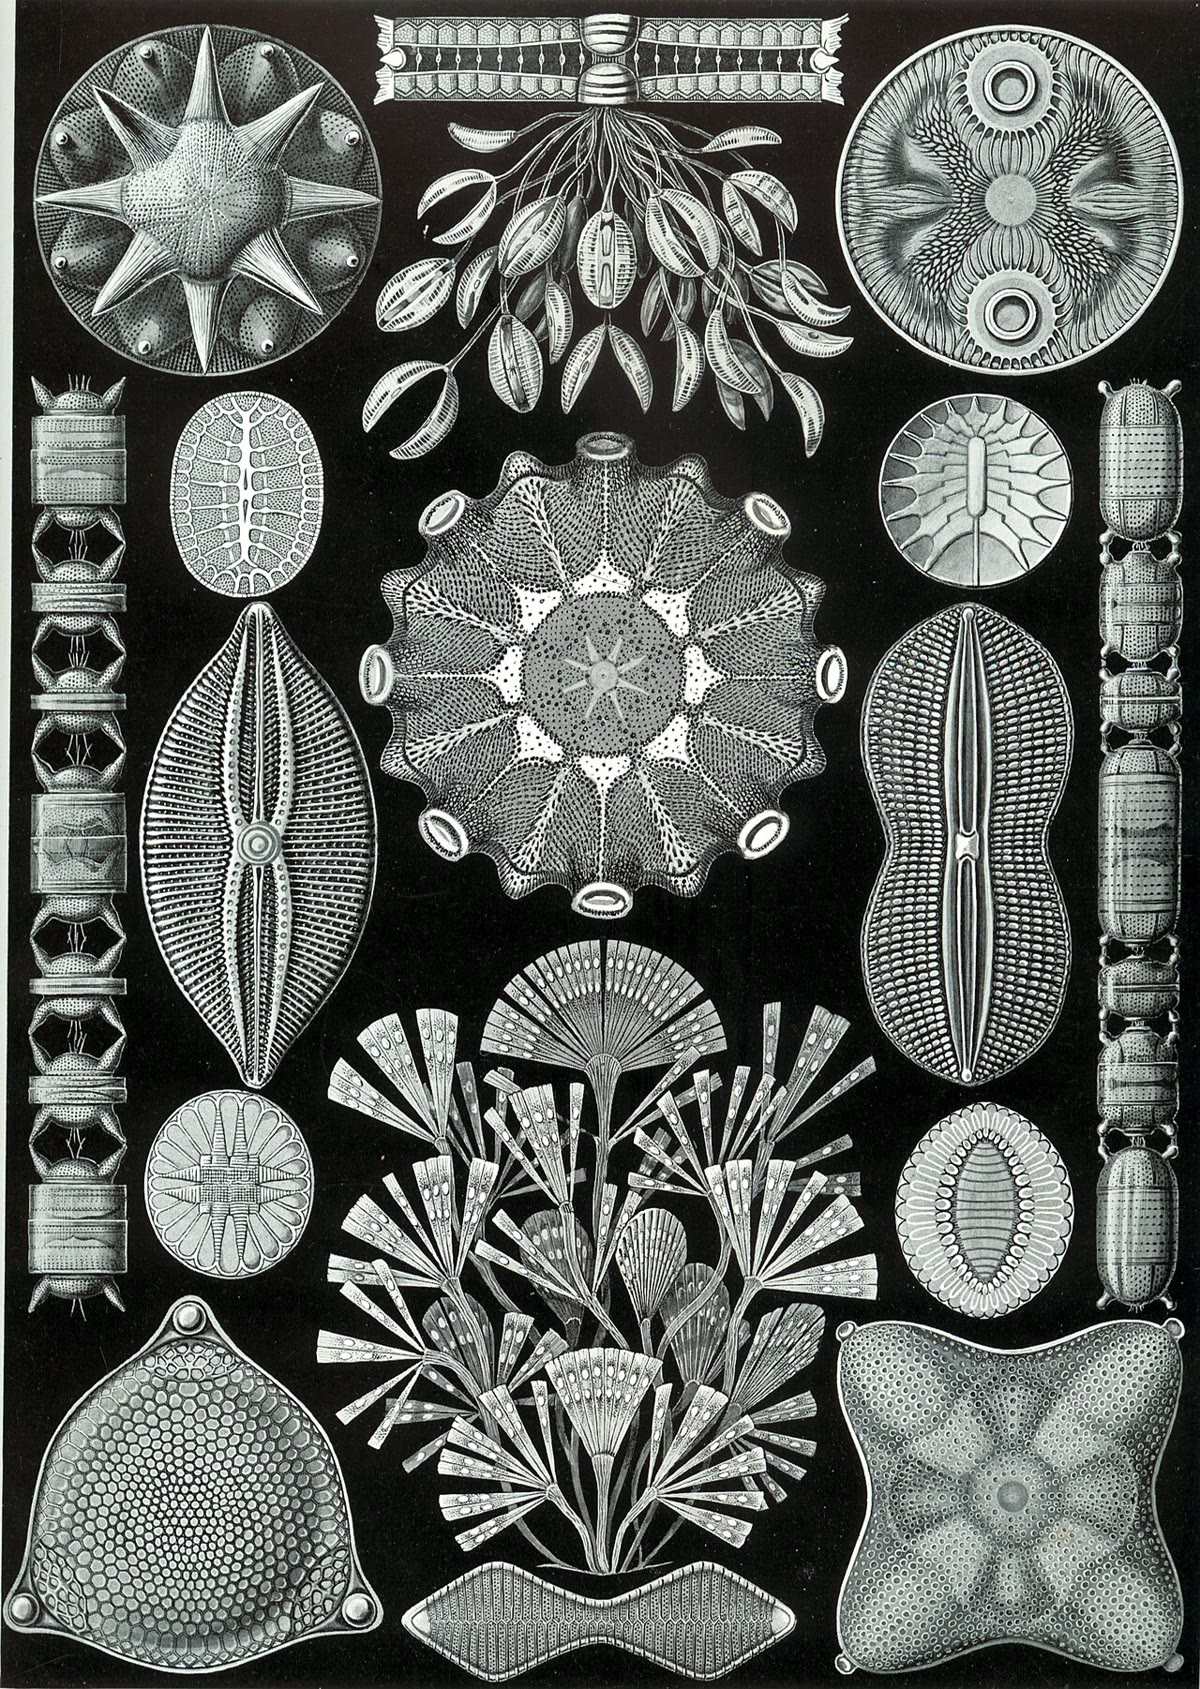
\includegraphics[width=0.36\linewidth]{images/book3/haeckel-diatomea.jpg}\hspace{0.03\linewidth}
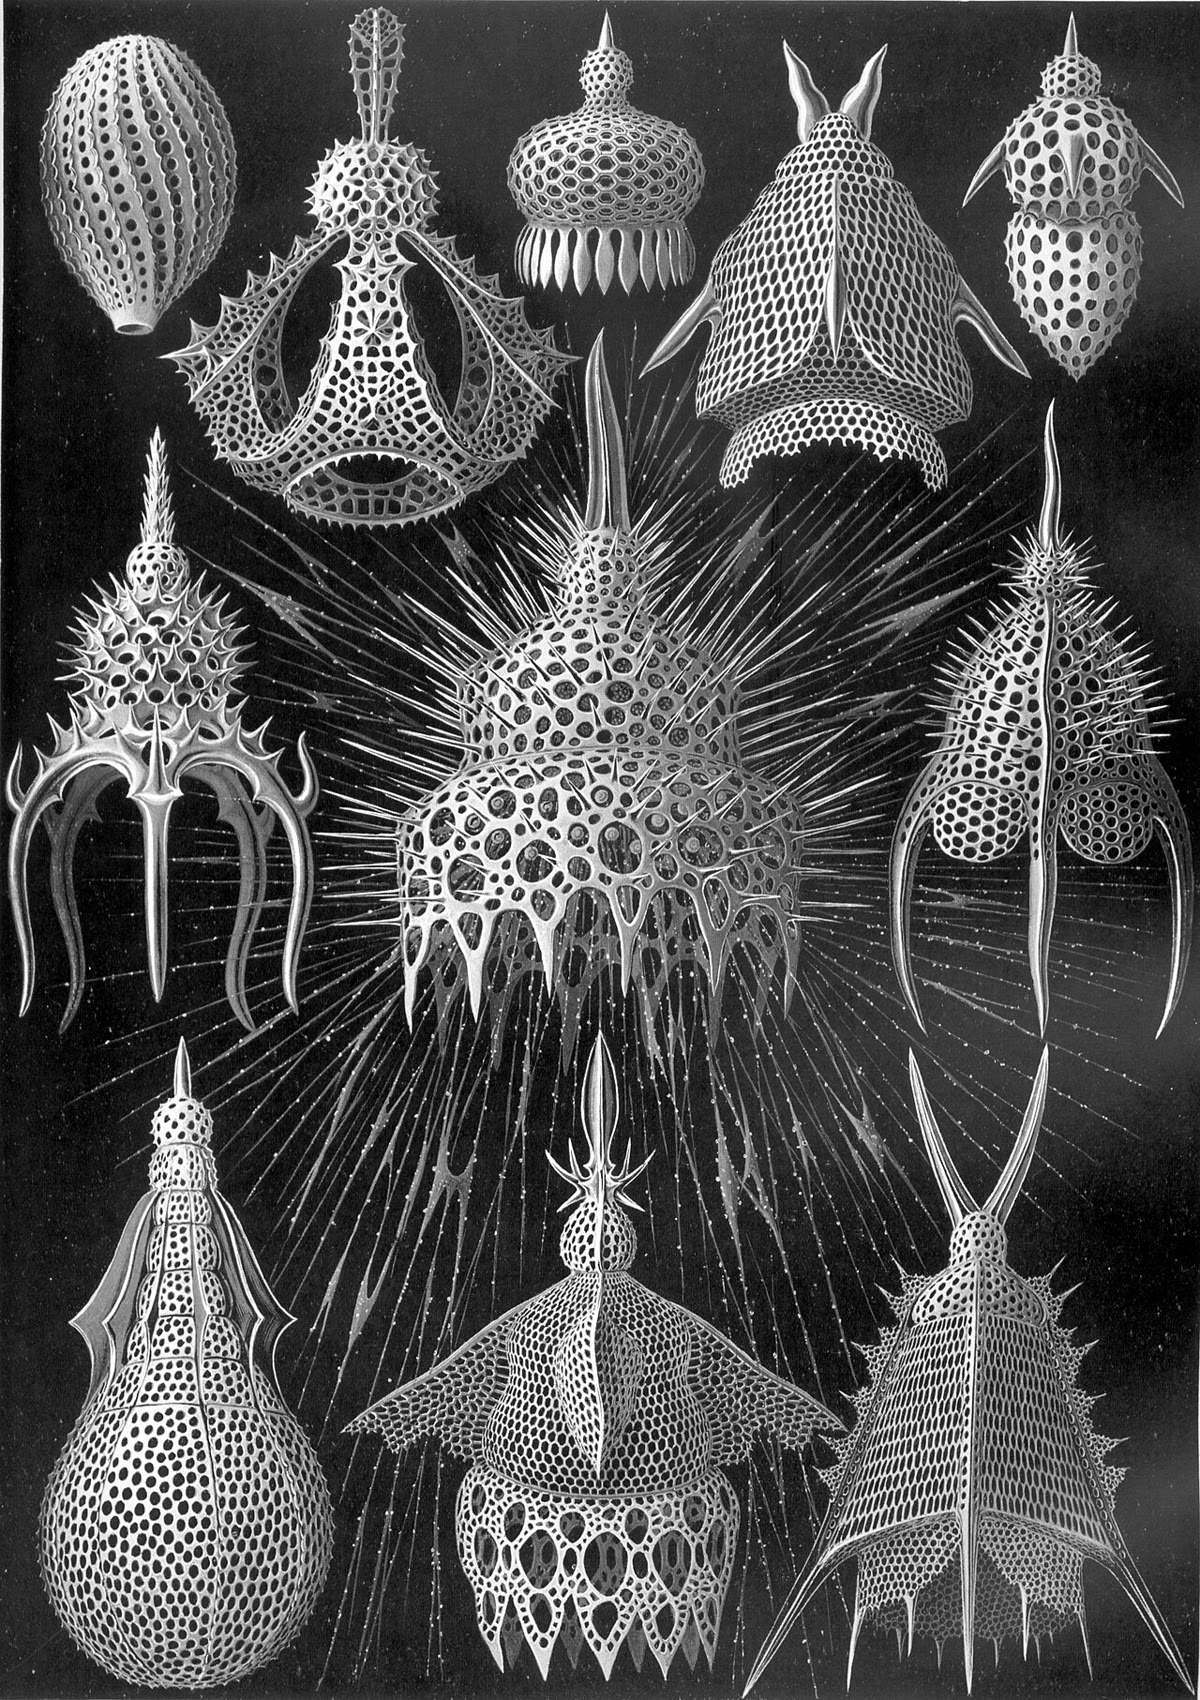
\includegraphics[width=0.36\linewidth]{images/book3/haeckel-cyrtoidea.jpg}

{\small \omterm{def:b1:cell-unit-of-life:prokeuk}{सुकेंद्रकियों} के दो ऐसे वंशक्रम जिनका कोई प्रचलित नाम नहीं है,
अर्न्स्ट हेकल के 1904 के पट्टों में: डायटम (स्ट्रामेनोपाइल, सिलिका के
कवचों में) और रेडिओलेरियन (राइज़ेरियन, सिलिका के कंकालों में)। हर समूह
दसियों हज़ार \omterm{def:b1:classifying-biodiversity:species}{जातियाँ} रखता है।}
\end{omfigure}

\section{जीवन की सूची}

\begin{definition}[जैव विविधता]\label{def:b1:classifying-biodiversity:biodiversity}
\index{जैव विविधता}\index{विलुप्ति}
\emph{जैव विविधता} हर स्तर पर जीवन की विविधता है: \omterm{def:b1:classifying-biodiversity:species}{जातियों} के भीतर जननिक
विविधता, \omterm{def:b1:classifying-biodiversity:species}{जातियों} की संख्या और बहुलता, तथा \omterm{def:b1:ecosystem-organization:ecosystem}{समुदायों} और पारितंत्रों की
विविधता। उसकी सूची अधूरी है: लगभग \num{2} लाख हज़ार \omterm{def:b1:classifying-biodiversity:species}{जातियों} का वर्णन हो
चुका है, जिनमें दस लाख कीट, \num{380000} पौधे, \num{150000} कवक,
\num{70000} कशेरुकी और मोलस्क, क्रस्टेशी, प्रोटिस्ट तथा \omterm{def:b1:cell-unit-of-life:prokeuk}{प्राक्केंद्रकी}
हर एक के कुछ दसियों हज़ार हैं; \omterm{def:b1:cell-unit-of-life:prokeuk}{सुकेंद्रकी} \omterm{def:b1:classifying-biodiversity:species}{जातियों} की संख्या, इस दर से कि
नए ऊँचे \omterm{def:b1:classifying-biodiversity:nomenclature}{वर्गक} अब भी कितनी तेज़ी से मिल रहे हैं, \num{9} लाख हज़ार के पास
आँकी जाती है, यानी अधिकांश \omterm{def:b1:classifying-biodiversity:species}{जातियाँ} अनामित हैं, और उनमें से अधिकांश छोटी
हैं, उष्णकटिबंधी हैं, या दोनों। \omterm{def:b1:classifying-biodiversity:species}{जातियाँ} हमेशा \emph{विलुप्त} होती रही हैं
--- जीवाश्मों से निकली पृष्ठभूमि दर प्रति दस लाख पर लगभग एक \omterm{def:b1:classifying-biodiversity:species}{जाति} प्रति
वर्ष है --- और आवास-हानि, दोहन, आक्रामक \omterm{def:b1:classifying-biodiversity:species}{जातियों} तथा जलवायु से चलती वर्तमान
दर उससे सौ से हज़ार गुनी आँकी जाती है।
\end{definition}

\begin{omfigure}
\begin{tikzpicture}
\begin{axis}[
  xbar, bar width=7pt,
  width=0.82\linewidth, height=6.8cm,
  axis x line=bottom, axis y line=left,
  xmin=0, xmax=1200, xlabel={वर्णित जातियाँ (हज़ार में)},
  xlabel style={font=\small, at={(axis description cs:0.5,-0.12)}, anchor=north},
  symbolic y coords={bacteria and archaea, mammals, birds, fishes, protists, molluscs, crustaceans, arachnids, fungi, land plants, insects},
  yticklabels={बैक्टीरिया और आर्किया, स्तनधारी, पक्षी, मछलियाँ, प्रोटिस्ट, मोलस्क, क्रस्टेशी, अष्टपादी, कवक, थलीय पौधे, कीट},
  ytick=data, tick label style={font=\small},
  enlarge y limits=0.06, xtick={0,200,400,600,800,1000},
  nodes near coords, nodes near coords style={font=\scriptsize, anchor=west},
]
\addplot[fill=omDef!40, draw=omDef] coordinates {(12,bacteria and archaea) (6.5,mammals) (11,birds) (35,fishes) (60,protists) (85,molluscs) (70,crustaceans) (110,arachnids) (150,fungi) (380,land plants) (1000,insects)};
\end{axis}
\end{tikzpicture}

{\small समूह के अनुसार वर्णित \omterm{def:b1:classifying-biodiversity:species}{जातियाँ}, हज़ार में (पूर्णांकित)। सारी
नामित \omterm{def:b1:classifying-biodiversity:species}{जातियों} का आधा कीट हैं, और \omterm{def:b1:cell-unit-of-life:prokeuk}{प्राक्केंद्रकियों} की --- जो किसी भी
आणविक माप से सबसे विविध \omterm{def:b1:organism-environment:organism}{जीव} हैं --- वर्णित \omterm{def:b1:classifying-biodiversity:species}{जातियाँ} स्तनधारियों और
पक्षियों को मिलाकर से भी कम हैं।}
\end{omfigure}

\begin{omfigure}
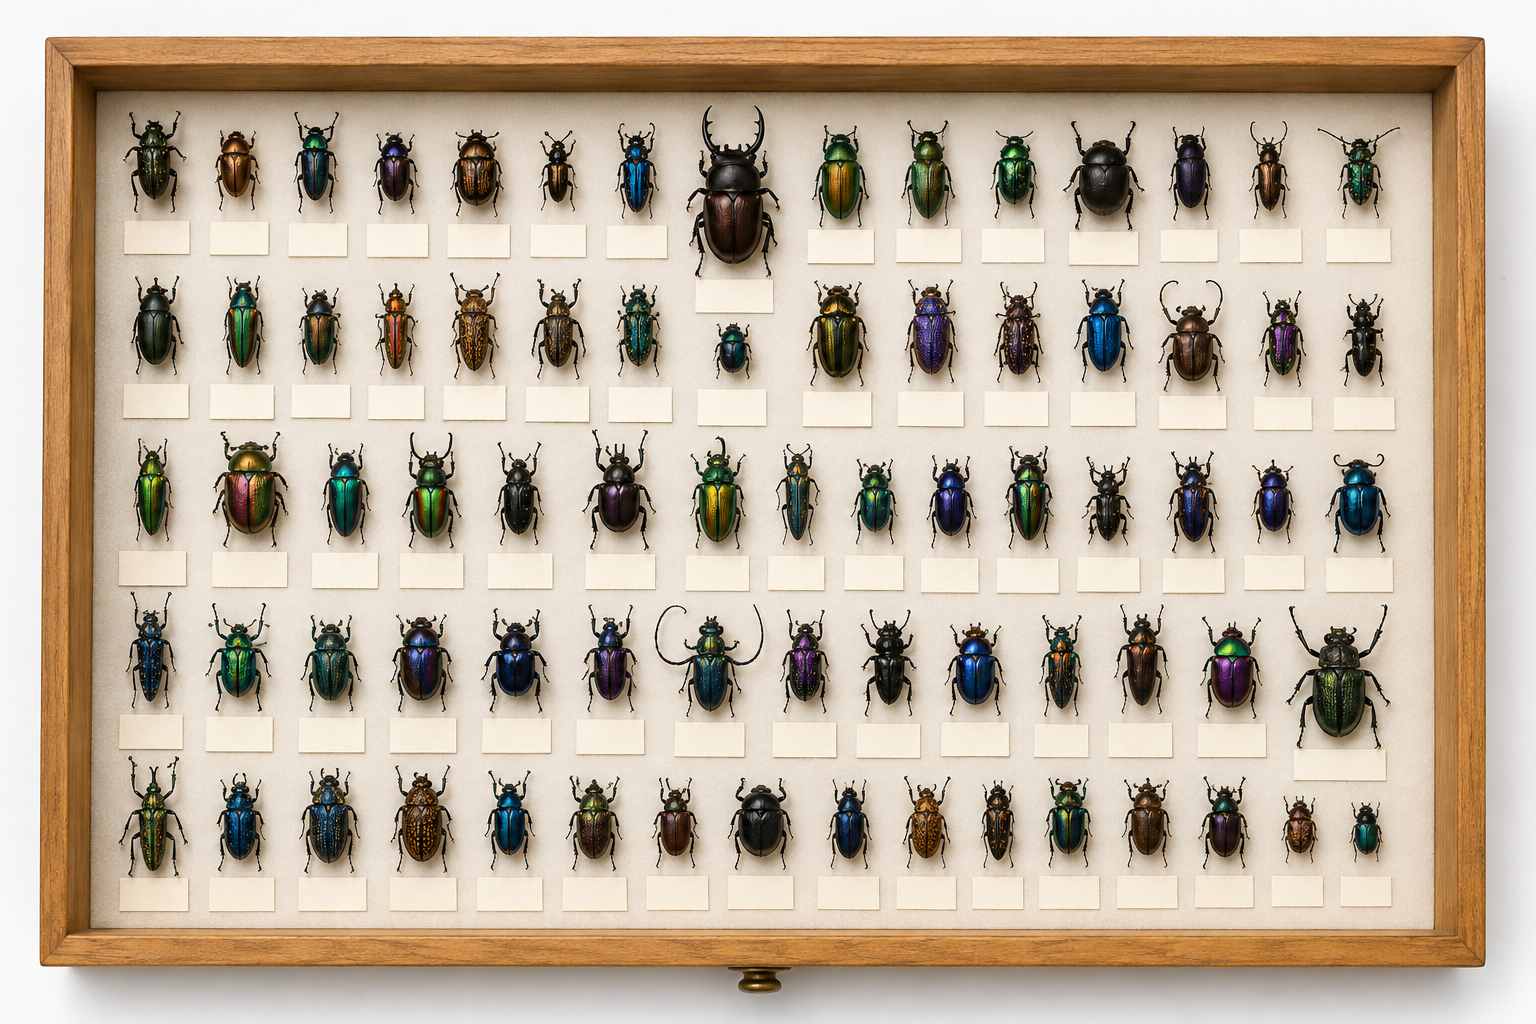
\includegraphics[width=0.56\linewidth]{images/book3/ai/b3-29-beetle-collection.png}

{\small पिन लगे भृंगों से भरी किसी संग्रहालय की दराज़: संग्रह ही सूची है,
और ऐसी एक दराज़ ऐसी \omterm{def:b1:classifying-biodiversity:species}{जातियाँ} रख सकती है जिनका नाम अब तक किसी ने नहीं
रखा।}
\end{omfigure}

\begin{method}[कितनी जातियाँ हैं इसका आकलन]\label{met:b1:classifying-biodiversity:estimate}
\begin{enumerate}
  \item किसी समूह में वर्णित \omterm{def:b1:classifying-biodiversity:species}{जातियाँ} और वह दर गिनिए जिससे नई अब भी जुड़
        रही हैं; यदि दर धीमी न पड़ रही हो, तो सूची पूरी होने से बहुत
        दूर है।
  \item किसी अच्छी तरह ज्ञात समूह से किसी कम ज्ञात समूह तक किसी अनुपात
        से बहिर्वेशन कीजिए: यदि शीतोष्ण प्राणिजात प्रति पादप \omterm{def:b1:classifying-biodiversity:species}{जाति} दो
        कीट \omterm{def:b1:classifying-biodiversity:species}{जातियाँ} रखते हों, और उष्णकटिबंध में \num{250000} पौधे हों,
        तो उष्णकटिबंध कम से कम पाँच लाख कीट रखता है।
  \item किसी छोटे क्षेत्र से गहनता से नमूने लीजिए (किसी उष्णकटिबंधी
        वृक्ष की छत्रछाया को कीटनाशक से धूम्रित करना, समुद्री जल के एक
        लीटर का \omterm{def:b1:nucleic-acids:chain}{DNA} अनुक्रमित करना) और नई निकली \omterm{def:b1:classifying-biodiversity:species}{जातियों} के अंश से ऊपर
        बढ़ाइए।
  \item कोटियों भर के ढर्रे का उपयोग कीजिए: संघों, वर्गों, गणों और कुलों
        की संख्याएँ लगभग पूरी हैं और जाति-स्तर की ओर नियमित रूप से
        चढ़ती हैं; उस नियमितता का बहिर्वेशन कुल संख्या देता है (लगभग
        \num{8.7} लाख हज़ार \omterm{def:b1:cell-unit-of-life:prokeuk}{सुकेंद्रकी})।
  \item आकलन को उसके परास के साथ बताइए; \omterm{def:b1:cell-unit-of-life:prokeuk}{प्राक्केंद्रकियों} के लिए ईमानदार
        उत्तर परिमाण की कई कोटियों का एक परास है।
\end{enumerate}
\end{method}

\section{अभ्यास}

\begin{exercise}[$\star$]\label{exo:b1:classifying-biodiversity:1}
घरेलू बिल्ली का नाम सही-सही लिखिए, उसका \omterm{def:b1:classifying-biodiversity:nomenclature}{वंश} और उसका विशेषण पहचानिए, और
उसे उसके कुल, गण, वर्ग तथा संघ में रखिए।
\end{exercise}

\begin{exercise}[$\star$]\label{exo:b1:classifying-biodiversity:2}
\omterm{def:b1:classifying-biodiversity:characters}{समजातता} और \omterm{def:b1:classifying-biodiversity:characters}{समवृत्तिता} की परिभाषा हर एक के एक उदाहरण के साथ दीजिए, और
बताइए कि कौन-सी किसी \omterm{def:b1:classifying-biodiversity:systematics}{क्लेड} का साक्ष्य है।
\end{exercise}

\begin{exercise}[$\star$]\label{exo:b1:classifying-biodiversity:3}
बताइए कि ``मछलियाँ'', ``पक्षी'' और ``गरम-खून वाले जंतु'' एकवंशज हैं,
अपूर्णवंशज या बहुवंशज, कारण के साथ।
\end{exercise}

\begin{exercise}[$\star$]\label{exo:b1:classifying-biodiversity:4}
तीनों अधिजगतों के नाम बताइए और आर्किया को बैक्टीरिया से अलग करते दो गुण
दीजिए।
\end{exercise}

\begin{exercise}[$\star\star$]\label{exo:b1:classifying-biodiversity:5}
\omterm{def:b1:classifying-biodiversity:species}{जैविक जाति संकल्पना} बैक्टीरिया पर या जीवाश्मों पर क्यों लागू नहीं हो
सकती, और उसकी जगह क्या बरता जाता है?
\end{exercise}

\begin{exercise}[$\star\star$]\label{exo:b1:classifying-biodiversity:6}
तीन \omterm{def:b1:classifying-biodiversity:nomenclature}{वर्गक} X, Y, Z और एक \omterm{def:b1:classifying-biodiversity:characters}{बाह्यसमूह}। लक्षण 1 X और Y में व्युत्पन्न है;
लक्षण 2 Y और Z में; लक्षण 3 X और Y में; लक्षण 4 X और
Y में। दोनों संभव वृक्ष खींचिए, उनकी लंबाइयाँ निकालिए, और सबसे मितव्ययी
वृक्ष तथा उसकी \omterm{def:b1:classifying-biodiversity:characters}{समवृत्तिता} बताइए।
\end{exercise}

\begin{exercise}[$\star\star$]\label{exo:b1:classifying-biodiversity:7}
कोई क्लेडोग्राम बनाने के लिए \omterm{def:b1:classifying-biodiversity:characters}{बाह्यसमूह} क्यों चाहिए, और यदि चुना गया
\omterm{def:b1:classifying-biodiversity:characters}{बाह्यसमूह} सचमुच समूह के भीतर ही आता हो तो क्या गड़बड़ हो जाती है?
\end{exercise}

\begin{exercise}[$\star\star$]\label{exo:b1:classifying-biodiversity:8}
समझाइए कि जंतु और कवक जंतुओं तथा पौधों की तुलना में अधिक निकट संबंधी
क्यों माने जाते हैं, और ऑपिस्थोकॉन्ट कौन-सा लक्षण साझा करते हैं।
\end{exercise}

\begin{exercise}[$\star\star$]\label{exo:b1:classifying-biodiversity:9}
वोइस ने पाया कि मेथैनोजन बाकी बैक्टीरिया से उतने ही भिन्न हैं जितने
\omterm{def:b1:cell-unit-of-life:prokeuk}{सुकेंद्रकियों} से। इसने बैक्टीरिया के भीतर किसी नए जगत के बजाय किसी नए
अधिजगत को क्यों उचित ठहराया?
\end{exercise}

\begin{exercise}[$\star\star\star$]\label{exo:b1:classifying-biodiversity:10}
कीटनाशक से धूम्रित की गई किसी उष्णकटिबंधी वृक्ष-छत्रछाया से भृंगों की
1200 \omterm{def:b1:classifying-biodiversity:species}{जातियाँ} मिलती हैं, जिनकी \qty{20}{\%} उसी वृक्ष-जाति के लिए विशिष्ट
हैं; भृंग छत्रछाया के कीटों के \qty{40}{\%} हैं, और छत्रछाया वृक्ष के
कीटों का दो-तिहाई रखती है; उष्णकटिबंधी वृक्षों की \num{50000} \omterm{def:b1:classifying-biodiversity:species}{जातियाँ}
हैं। उष्णकटिबंधी कीट \omterm{def:b1:classifying-biodiversity:species}{जातियों} की संख्या आँकिए और मान्यताएँ गिनाइए।
\end{exercise}

\begin{exercise}[$\star\star\star$]\label{exo:b1:classifying-biodiversity:11}
किसी \omterm{def:b1:classifying-biodiversity:species}{जाति} का वर्णन संग्रहालय के एक ही नमूने से होता है; बाद में ऐसी जीवित
\omterm{def:b1:populations:population}{आबादियाँ} मिलती हैं जो ज़रा भिन्न हैं। यह तय करने में प्ररूप नमूने की
भूमिका समझाइए कि वह नाम किस पर लागू होता है, और यह भी कि वरीयता क्यों
मायने रखती है।
\end{exercise}

\begin{exercise}[$\star\star\star$]\label{exo:b1:classifying-biodiversity:12}
``\omterm{def:b1:classifying-biodiversity:parsimony}{मितव्ययिता} यह मानकर चलती है कि विकास सबसे छोटा रास्ता लेता है।''
विवेचना कीजिए: \omterm{def:b1:classifying-biodiversity:parsimony}{मितव्ययिता} सचमुच क्या मानकर चलती है, वह कब विफल होती है
(अभिसरण, तेज़ विकसित होते वंशक्रम), और किसी वृक्ष को जाँचने के लिए आणविक
आँकड़े तथा जीवाश्म कैसे बरते जाते हैं।
\end{exercise}

\section{समस्या: आठ कशेरुकी और एक वृक्ष}

\begin{problem}[{सप्ताहांत समस्या --- आठ कशेरुकियों का एक लक्षण-आव्यूह,
हाथ से बनाया उसका क्लेडोग्राम, मितव्ययिता से अंकित दो प्रतिद्वंद्वी वृक्ष,
एकवंशजता के लिए परखे गए पारंपरिक समूह, और एक जाति-गणना का आकलन, और अंत में
सबसे मितव्ययी वृक्ष तथा उसकी लंबाई}]
\label{pb:b1:classifying-biodiversity:1}
यह आव्यूह किसी लैम्प्रे (\omterm{def:b1:classifying-biodiversity:characters}{बाह्यसमूह}), किसी शार्क, किसी ट्राउट, किसी
फुफ्फुसमीन, किसी मेंढक, किसी छिपकली, किसी चूहे और किसी कबूतर के लिए दस
लक्षण अंकित करता है (1 = व्युत्पन्न अवस्था उपस्थित)।

\begin{center}
\footnotesize
\begin{tabular}{l*{10}{c}}
\hline
 & 1 & 2 & 3 & 4 & 5 & 6 & 7 & 8 & 9 & 10 \\
 & \rotatebox{90}{जबड़े} & \rotatebox{90}{अस्थिल कंकाल} & \rotatebox{90}{फेफड़े} & \rotatebox{90}{चार अंग} & \rotatebox{90}{उल्ब अंडा} & \rotatebox{90}{रोम} & \rotatebox{90}{पंख} & \rotatebox{90}{द्विगर्ती खोपड़ी} & \rotatebox{90}{ऊष्मारक्तता} & \rotatebox{90}{केरातिन शल्क} \\
\hline
लैम्प्रे & 0 & 0 & 0 & 0 & 0 & 0 & 0 & 0 & 0 & 0 \\
शार्क & 1 & 0 & 0 & 0 & 0 & 0 & 0 & 0 & 0 & 0 \\
ट्राउट & 1 & 1 & 0 & 0 & 0 & 0 & 0 & 0 & 0 & 0 \\
फुफ्फुसमीन & 1 & 1 & 1 & 0 & 0 & 0 & 0 & 0 & 0 & 0 \\
मेंढक & 1 & 1 & 1 & 1 & 0 & 0 & 0 & 0 & 0 & 0 \\
छिपकली & 1 & 1 & 1 & 1 & 1 & 0 & 0 & 1 & 0 & 1 \\
चूहा & 1 & 1 & 1 & 1 & 1 & 1 & 0 & 0 & 1 & 0 \\
कबूतर & 1 & 1 & 1 & 1 & 1 & 0 & 1 & 1 & 1 & 1 \\
\hline
\end{tabular}
\end{center}

\medskip
\noindent\textbf{भाग I --- आव्यूह पढ़ना।}
\begin{enumerate}
  \item \omterm{def:b1:classifying-biodiversity:characters}{बाह्यसमूह} को छोड़ सारे \omterm{def:b1:classifying-biodiversity:nomenclature}{वर्गक} कौन-से लक्षण साझा करते हैं? वे
        वृक्ष के बारे में क्या बताते हैं?
  \item लक्षणों को इस क्रम में गिनाइए कि व्युत्पन्न अवस्था कितने \omterm{def:b1:classifying-biodiversity:nomenclature}{वर्गक}
        साझा करते हैं, और बताइए कि हर एक कौन-सा \omterm{def:b1:classifying-biodiversity:systematics}{क्लेड} परिभाषित करता है।
  \item कौन-से लक्षण किसी एक ही \omterm{def:b1:classifying-biodiversity:nomenclature}{वर्गक} में उपस्थित हैं? क्या वे उस \omterm{def:b1:classifying-biodiversity:nomenclature}{वर्गक}
        को रखने में कुछ काम के हैं?
  \item लक्षणों का कौन-सा जोड़ा आपस में टकराता है, और किन तीन \omterm{def:b1:classifying-biodiversity:nomenclature}{वर्गकों} के
        बीच?
  \item लक्षण 3 (फेफड़े) की ध्रुवता बताइए और समझाइए कि \omterm{def:b1:classifying-biodiversity:characters}{बाह्यसमूह} उसे
        कैसे तय करता है।
  \item बाकी वृक्ष तय हो जाने पर तीनों उल्बधारियों को आपस में जोड़ने
        वाले कितने भिन्न मूलित वृक्ष हो सकते हैं? इस चुनाव पर कौन-से
        लक्षण असर डालते हैं?
\end{enumerate}

\medskip
\noindent\textbf{भाग II --- वृक्ष बनाना।}
\begin{enumerate}[resume]
  \item लक्षण 1 से 5 तक के निहित क्लेडोग्राम को खींचिए: जबड़ों से उल्ब
        अंडे तक बसे हुए \omterm{def:b1:classifying-biodiversity:systematics}{क्लेड}।
  \item उल्बधारियों के भीतर वृक्ष A खींचिए, जिसमें छिपकली और कबूतर
        सहोदर \omterm{def:b1:classifying-biodiversity:nomenclature}{वर्गक} हैं, और वृक्ष B, जिसमें चूहा और कबूतर सहोदर हैं।
  \item वृक्ष A की लंबाई निकालिए: दसों लक्षणों में से हर एक के लिए वे
        न्यूनतम बदलाव जो उसे चाहिए।
  \item वृक्ष B की लंबाई भी वैसे ही निकालिए।
  \item कौन-सा वृक्ष सबसे मितव्ययी है, और कितने से?
  \item वरीय वृक्ष पर समवृत्त लक्षण का नाम बताइए और उसकी विकासीय
        व्याख्या दीजिए।
  \item यदि लक्षण 8 और 10 हटा दिए जाएँ, तो दोनों लंबाइयाँ क्या होतीं,
        और आप क्या निष्कर्ष निकालते?
\end{enumerate}

\medskip
\noindent\textbf{भाग III --- वृक्ष पर समूह।}
\begin{enumerate}[resume]
  \item वरीय वृक्ष पर क्या समूह (शार्क, ट्राउट, फुफ्फुसमीन)
        --- यानी ``मछलियाँ'' --- एकवंशज है? कौन-सा \omterm{def:b1:classifying-biodiversity:nomenclature}{वर्गक} जोड़ना पड़ता?
  \item क्या (छिपकली, चूहा, कबूतर), यानी उल्बधारी, एकवंशज हैं? उनका
        \omterm{def:b1:classifying-biodiversity:characters}{सहव्युत्पन्न लक्षण} बताइए।
  \item कबूतर के रख दिए जाने पर क्या अकेली (छिपकली) जोड़ मगरमच्छ तथा
        कछुए --- यानी पारंपरिक ``सरीसृप'' --- एकवंशज हैं? वह कैसा समूह
        है?
  \item क्या ऊष्मारक्तता से समूहबद्ध (चूहा, कबूतर) एक \omterm{def:b1:classifying-biodiversity:systematics}{क्लेड} है? वह कैसा
        समूह है?
  \item फुफ्फुसमीन को अक्सर मछली कहा जाता है। वृक्ष पर वह ट्राउट के पास
        है या मेंढक के? कौन-सा लक्षण तय करता है?
  \item किसी लिनियन वर्गीकरण में तीनों उल्बधारी जिन कोटियों में बैठते वे
        बताइए, और समझाइए कि वे कोटियाँ उनके विभाजनों की गहराई के बारे
        में कोई सूचना क्यों नहीं देतीं।
\end{enumerate}

\medskip
\noindent\textbf{भाग IV --- सूची।}
\begin{enumerate}[resume]
  \item कशेरुकियों की लगभग \num{70000} \omterm{def:b1:classifying-biodiversity:species}{जातियाँ} वर्णित हैं और नए वर्णनों
        की दर मछलियों के लिए साल में \num{300} और स्तनधारियों के लिए
        \num{20} है। कौन-सी सूची पूरी होने के अधिक पास है?
  \item समुद्री जल के \qty{1}{L} में \omterm{def:b1:nucleic-acids:chain}{DNA} के किसी सर्वेक्षण को
        \num{2000} भिन्न राइबोसोमी अनुक्रम मिलते हैं, जिनमें से
        \qty{90}{\%} किसी वर्णित \omterm{def:b1:organism-environment:organism}{जीव} से मेल नहीं खाते। इसका
        \omterm{def:b1:cell-unit-of-life:prokeuk}{प्राक्केंद्रकी} सूची के लिए क्या अर्थ है?
  \item यदि पृष्ठभूमि \omterm{def:b1:classifying-biodiversity:biodiversity}{विलुप्ति} दर प्रति दस लाख पर एक \omterm{def:b1:classifying-biodiversity:species}{जाति} प्रति वर्ष हो
        और \omterm{def:b1:cell-unit-of-life:prokeuk}{सुकेंद्रकी} \omterm{def:b1:classifying-biodiversity:species}{जातियाँ} \num{9} लाख हज़ार हों, तो साल में कितनी
        विलुप्त होनी चाहिए? अच्छी तरह अध्ययन किए गए समूहों के लिए देखी
        गई दर लगभग \num{1000} गुना ऊँची है: वह सारे \omterm{def:b1:cell-unit-of-life:prokeuk}{सुकेंद्रकियों} के
        लिए साल में कितनी देती है?
  \item वर्णित होने से पहले विलुप्त हो जाने वाली कोई \omterm{def:b1:classifying-biodiversity:species}{जाति} \omterm{def:b1:ecosystem-organization:ecosystem}{पारितंत्र} के
        साथ-साथ \omterm{def:b1:classifying-biodiversity:systematics}{वर्गिकी} के लिए भी हानि क्यों है?
  \item समझाइए कि वर्णित कुलों की संख्या कुल संख्या का वर्णित \omterm{def:b1:classifying-biodiversity:species}{जातियों} की
        संख्या से बेहतर मार्गदर्शक क्यों है।
  \item परिणाम बताइए: आठ कशेरुकियों का सबसे मितव्ययी वृक्ष, बसे हुए
        कोष्ठकों में लिखा हुआ, और उसकी लंबाई।
\end{enumerate}
\end{problem}
